\documentclass[12pt]{beamer}
\usetheme{Boadilla}

\usepackage[utf8]{inputenc}
\usepackage[T1]{fontenc}
\usepackage[francais]{babel}
\usepackage{amsmath}
\usepackage{amsfonts}
\usepackage{amssymb}
\usepackage{graphicx}

\setbeamertemplate{enumerate items}[square]

\author{Thomas \textsc{Citharel}}
\title{Soutenance de stage}
\subtitle{Développement et mise en place d'une application de gestion d'agendas}
\logo{}
\institute{IUT d'Orléans}
\date{31 août 2015}
\subject{sujet}
\setbeamercovered{transparent}
\setbeamertemplate{navigation symbols}{}

\begin{document}
	\maketitle
	
	\begin{frame}
		\frametitle{Sommaire}
		\tableofcontents
	\end{frame}
	\begin{frame}
		\frametitle{Présentation de la structure}
		\begin{figure}
		\centering
		
\includegraphics[width=0.2\linewidth]{images/Framasoft-Logo}
		\caption{Logo de Framasoft}
		\label{fig:framasoft-logo}
		\end{figure}

		\section{Présentation de la structure}
		\subsection{Historique}
	\end{frame}
	\begin{frame}
		\frametitle{Présentation de la structure}
		\begin{figure}
			\centering
			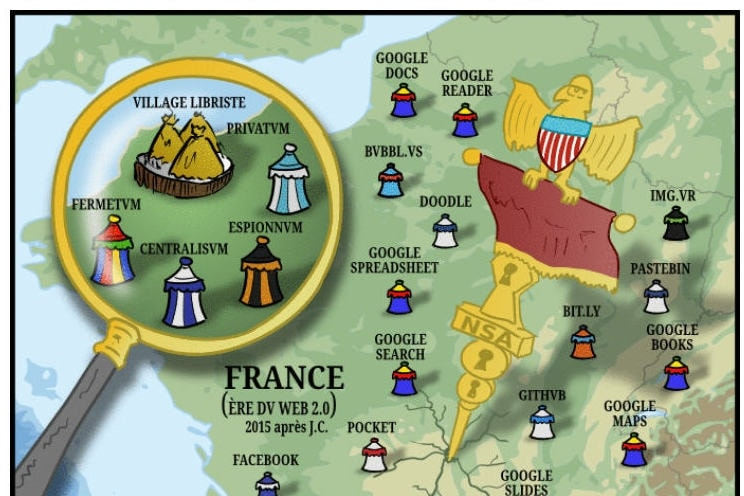
\includegraphics[width=0.3\linewidth]{images/degooglisons-internet}
			\caption{Carte de la campagne Dégooglisons}
			\label{fig:degooglisons-carte}
		\end{figure}
		
		\subsection{Liste des services}
		
		\centering
		\begin{tabular}{|l|l|}
			\hline
			Service en ligne & Alternative \\
			\hline
			Google Docs & Framapad \\
			\hline
			Google Spreadsheet & Framacalc \\
			\hline
			Doodle & Framadate \\
			\hline
			Pocket & Framabag \\
			\hline
		\end{tabular}
	\end{frame}
	\section{Présentation du projet}
	\begin{frame}
		\frametitle{Présentation du projet}
		\subsection{Alternative à Google Agenda}
		\begin{figure}
				\centering
				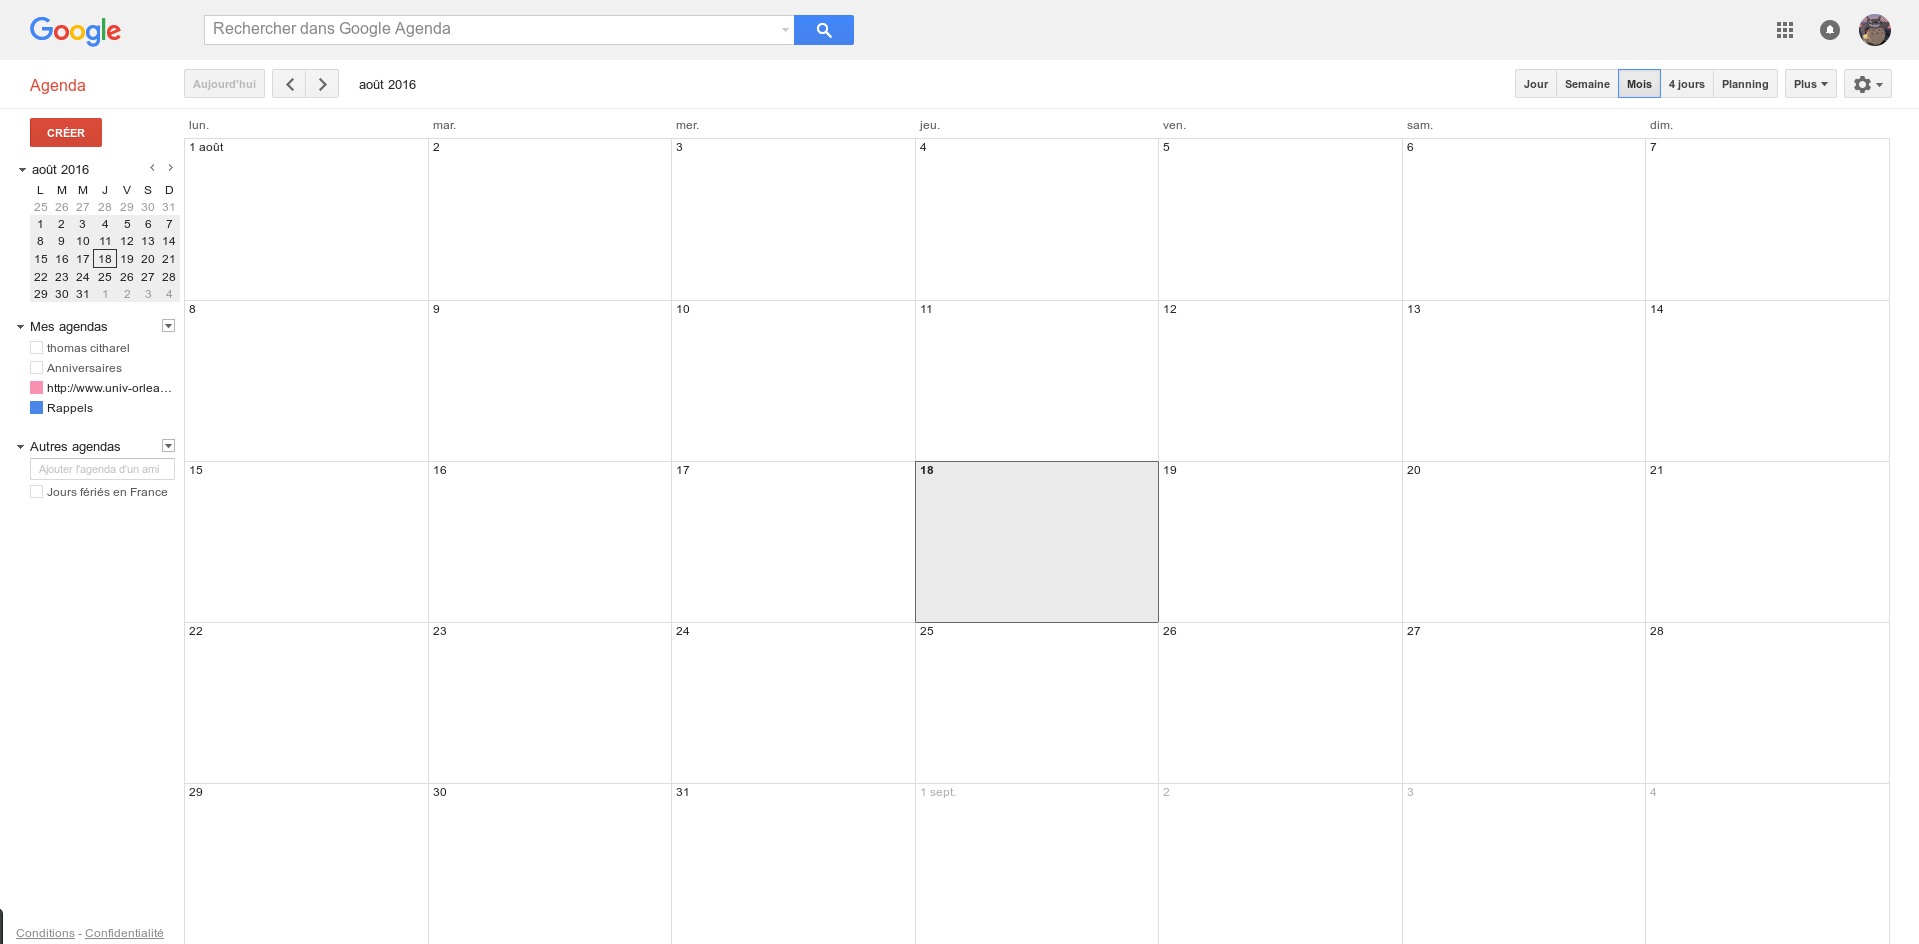
\includegraphics[width=0.7\linewidth]{images/google-agenda-interface-actuelle}
				\caption{Aperçu de Google Agenda}
				\label{fig:google-agenda-interface-actuelle}
			\end{figure}
		\end{frame}
		\begin{frame}
		\frametitle{Présentation du projet}
		Solution basée sur ownCloud et son application Calendar.
		\begin{itemize}
			\visible<1->{\item Créée en \textbf{2008}}
			\visible<2->{\item Écrit en \textbf{PHP}}
			\visible<3->{\item Fonctionnement autour d'un cœur et d'un ensemble d'applications}
		\end{itemize}
		\end{frame}
		\subsection{L'application existante}
		\begin{frame}
		\frametitle{Présentation du projet}
			Fonctionnalités existantes
			\begin{enumerate}
				\visible<1->{\item Gestion de la liste d'agendas}
				\visible<2->{\item Gestion d'événements}
				\visible<3->{\item Partage d'événements}
				\visible<4->{\item Synchronisation avec applications clientes}
				\visible<5->{\item Import/Export d'agendas}
			\end{enumerate}
	\end{frame}
	\section{Objectifs du stage}
	\begin{frame}
		\frametitle{Objectifs du stage}
		\begin{enumerate}
		\visible<1->{\item Ajout de fonctionnalités}
		\begin{enumerate}
			\visible<2->{\item Publication d'un calendrier}
			\visible<3->{\item Abonnement à des calendriers}
		\end{enumerate}
		\visible<3->{\item Mise en place du service}
		\visible<4->{\item Rédaction de la documentation}
	\end{enumerate}
	\end{frame}
	\section{Réalisation du projet}
	\begin{frame}
		\frametitle{Réalisation du projet}
		\begin{itemize}
			\visible<1->{\item Utilisation de l'éditeur Atom, de PHP et de SQLite.}
			\visible<2->{\item Mise en place sur VM pour tests utilisateur}
			\visible<3->{\item Tests pratiques avec applications clientes}
		\end{itemize}
	\end{frame}
	\begin{frame}
		\frametitle{Bilan}
		\section{Bilan}
	\end{frame}
\end{document}